\documentclass[MASTER.tex]{subfiles} 
\begin{document} 
	
	
\begin{frame}
	\huge
\[ \mbox{Other Interesting Python Packages} \]
\end{frame}

%===========================================================%
\begin{frame}
	\frametitle{statsmodels}
	\large
	\begin{itemize}
	\item \texttt{statsmodels} provides a large range of cross-sectional models aswell assometime-series models. 
	\item statsmodels
	uses a model descriptive language (provided via the Python package patsy) to formulate the model
	when working with pandas \texttt{DataFrames}.
	\item Models supported include linear regression, generalized linear
	models, limited dependent variable models, ARMA and VAR models.
	\end{itemize}
\end{frame}

%===========================================================%
\begin{frame}
	\frametitle{Bokeh Data Visualization}
		\begin{figure}
\centering
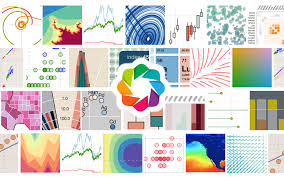
\includegraphics[width=1.0\linewidth]{bokehlogo}
\end{figure}

\end{frame}
%===========================================================%
\begin{frame}
	\frametitle{Bokeh Data Visualization}

\begin{figure}
\centering
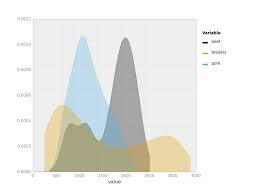
\includegraphics[width=1.0\linewidth]{bokehplot}

\end{figure}
	
\end{frame}
%===========================================================%
\begin{frame}
	\frametitle{Bokeh Data Visualization}
	\textbf{Bokeh Data Visualization}
	\begin{itemize}
		\item interactive graphics for the web
		\item designed for large data sets
		\item Designed for streaming data
		\item Native interface in pythin
		\item Fast javascript components
		\item DARPA funded
		\item v.01 relase imminent
	\end{itemize}
	
\end{frame}


\begin{frame}
	\begin{figure}
\centering

\includegraphics[width=0.7\linewidth]{SKL-logo}

\end{figure}

\end{frame}
%===========================================================%

\begin{frame}
	\frametitle{scikit.learn}
		\begin{figure}
			\centering
			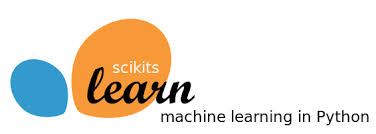
\includegraphics[width=0.5\linewidth]{SKL-logo2}
		
		\end{figure}
		
	\begin{itemize}
	\item scikit-learn is an open source machine learning library for the Python programming language. 
	\item scikit-learn features various classification, regression and clustering algorithms including support vector machines, logistic regression, naive Bayes, random forests, gradient boosting, k-means and DBSCAN. \item scikit-learn is designed to interoperate with the Python numerical and scientific libraries NumPy and SciPy.
	\end{itemize}
\end{frame}
%===========================================================%
\begin{frame}
\textbf{Sci-Kit Learn Site info}
	\begin{figure}
\centering
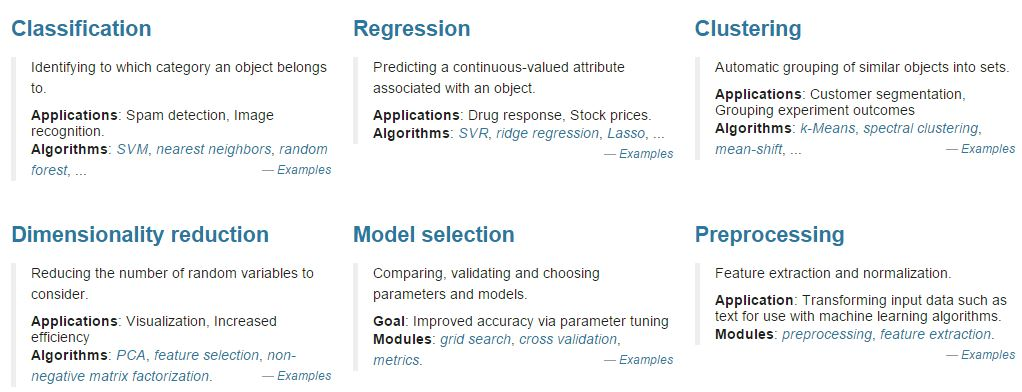
\includegraphics[width=1.1\linewidth]{SKLsiteinfo}
\end{figure}
\end{frame}
%===========================================================%
\begin{frame}
\begin{figure}
\centering
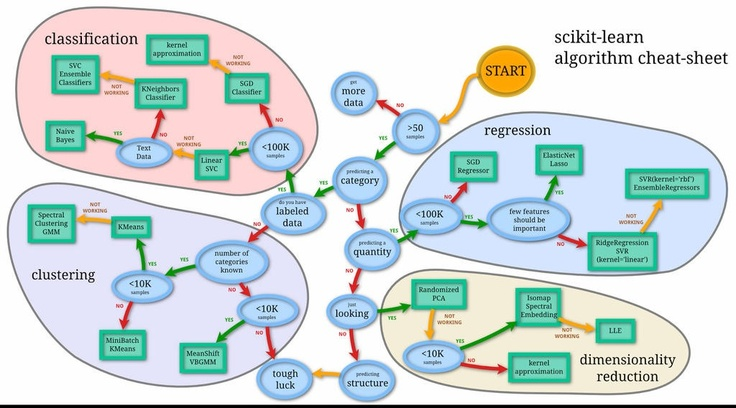
\includegraphics[width=0.9\linewidth]{SKLCheatSheet}

\end{figure}
\end{frame}
%===========================================================%
\begin{frame}
	\begin{figure}
		\centering
		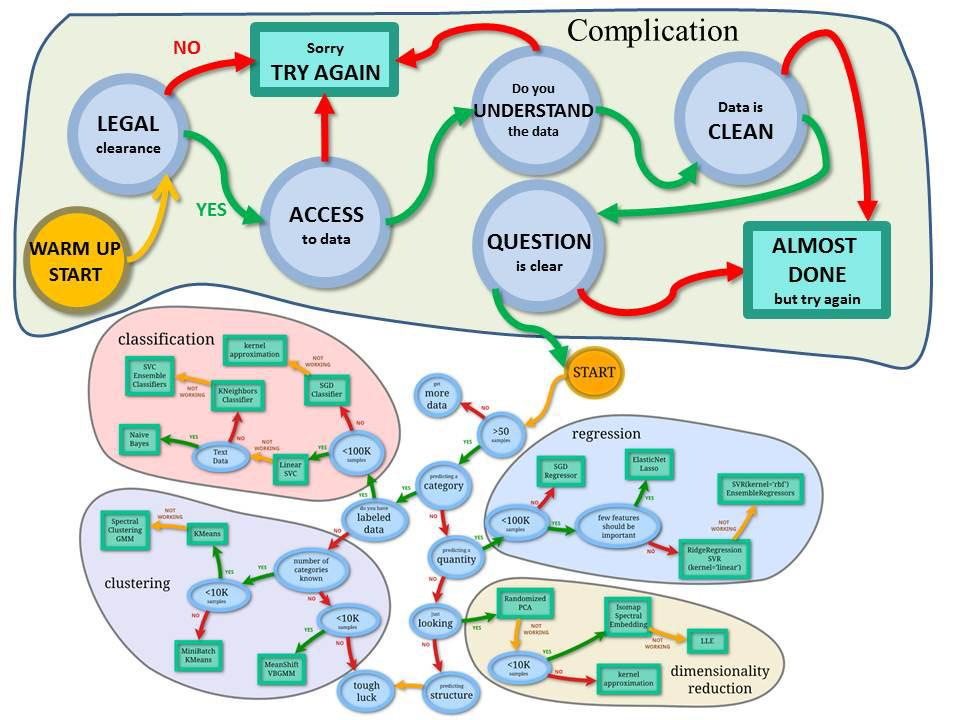
\includegraphics[width=0.9\linewidth]{SKLCheatSheet2}
		
	\end{figure}
\end{frame}
\begin{frame}

\end{frame}
\begin{frame}
	\begin{figure}
\centering
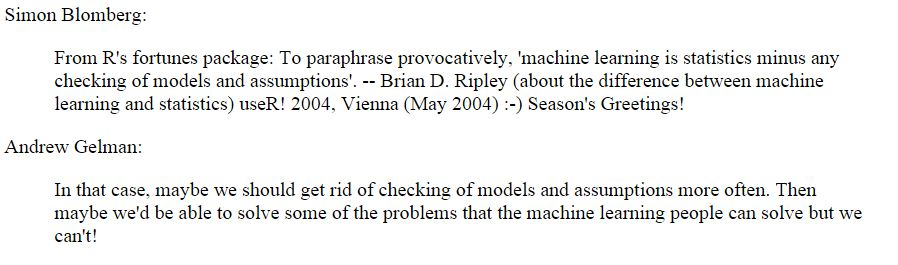
\includegraphics[width=1.1\linewidth]{machinelearningquotes}
\end{figure}
\Large Machine Learning is statistics minus any checking of models or assumptions
\end{frame}
%============================%
\begin{frame}
	\frametitle{The Data Science Profession}
	Data Science Retreat (Berlin)
	\begin{quote}
		MOOC have not  decreased the barrier of entry to machine-learning.
		
		
		Nowadays, you cannot be 'the guy who knows how to run (insert off-the-shelf-algo-here)'. 
		
		
		In dataland, that's the equivalent to being a code monkey. MOOCs and superb libraries (scikit-learn, R's ecosystem) made 
		sure there is plenty of people who can throw say a random forest to a problem. In the modern world, this is not adding that much value. 
	\end{quote}
\end{frame}
%===========================================================%
\begin{frame}
\frametitle{Other Packages}
\large
\textbf{pytz and babel}\\
ptyz and babel provide extended support for time zones and formatting information.\\ \bigskip
\textbf{rpy2 }\\
rpy2 provides an interface for calling R 3.0.x in Python, as well as facilities for easily moving data between
the two platforms.\\ \bigskip
\textbf{PyTables and h5py }\\
PyTables and h5py both provide access to HDF5 files, a flexible data storage format optimized for numeric
data.
\end{frame}
\end{document}